\documentclass{article}
\usepackage{graphicx} % Required for inserting images
\usepackage[utf8]{inputenc}
\usepackage[T2A]{fontenc}
\usepackage{amsmath}
\usepackage{pgfplots}
\usepackage{longtable}
\usepackage{tabularx}
\usepackage{makecell}
\usepackage{array}
\usepackage{indentfirst}
\usepackage{icomma}
\usepackage{geometry}
\usepackage{booktabs}
\usepackage{multirow}
\usepackage{multicol}
\usepackage{float}
\usepackage{diagbox}
\usepackage{gensymb}
\geometry{a4paper, margin=1in}

\renewcommand{\figurename}{Изображение}
\renewcommand{\tablename}{Таблица}

\title{Лабораторная работа №2.02

Определение отношения теплоемкостей воздуха при постоянных давлении и объеме}
\author{Топунов Антон, Z3142}
\date{21.02.2026}

\begin{document}

\maketitle
\clearpage
\section{Цели и задачи}
\subsection{Цели}
\begin{enumerate}
    \item Определение показателя адиабаты $\gamma = \frac{ C_p}{ C_v}$
\end{enumerate}
\subsection{Задачи}
\begin{enumerate}
    \item Провести измерение избыточных давлений в баллоне
    \item Рассчитать значение показателя адиабаты
\end{enumerate}
\section{Теоретическое введение}
Показатель адиабаты в одном опыте:
\begin{gather*}
    \gamma_i = \frac{ P_{2i}}{ P_{2i} - P_{1i}}
\end{gather*}
\begin{itemize}
    \item $P_{2i}$ - избыточное давление в баллоне сразу после накачки воздуха
    \item $P_{1i}$ - установившееся избыточное давление в баллоне 
\end{itemize}
Здесь под словом избыточное подразумевается разность давлений воздуха в баллоне и атмосферного давления.

Среднее значение $\gamma$:
\begin{gather*}
    \gamma = \frac{ \sum\limits_{ i=1}^{ N}\gamma_i}{ N}\\
    \Delta \gamma = \sqrt{(\Delta \gamma_\text{сл})^2 + ( \frac{ 2}{ 3}\Delta \gamma_\text{сист})^2}\\
    \Delta \gamma_\text{сл} = t_{\alpha , N} \cdot \sqrt{\frac{ \sum\limits_{i = 1 }^{N }{(\gamma_i-\gamma)^2}}{ N(N-1)}}\\
    \Delta \gamma_\text{сист} = \gamma\cdot \sqrt{\bigg(\Delta P \cdot \bigg(
        \frac{ 1}{ P_2} + \frac{ 1}{ P_2 - P_1}
        \bigg)\bigg)^2 + \bigg(\Delta P \cdot \bigg(
        \frac{ 1}{ P_2 - P_1}
        \bigg)\bigg)^2}
\end{gather*}
\begin{itemize}
    \item $P_2$ и $P_1$ - средние значения избыточных давлений
    \item $\Delta P$ - погрешность измерений давления
\end{itemize}
\section{Схема установки}
В данной лабораторной работе воздух многократно изотермически накачивается с помощью компрессора (1) в
баллон (2), после чего снимается показание разности давлений $P_2$ (3). После этого баллон
посредством "пружинного клапана" кратковременно соединяется с атмосферой (4).
После этого мы дожидаемся выравнивания давления и снимаем показание разности давлений $P_1$ (3).
Опыт повторяется несколько раз.

\begin{figure}[H]
   \centering
    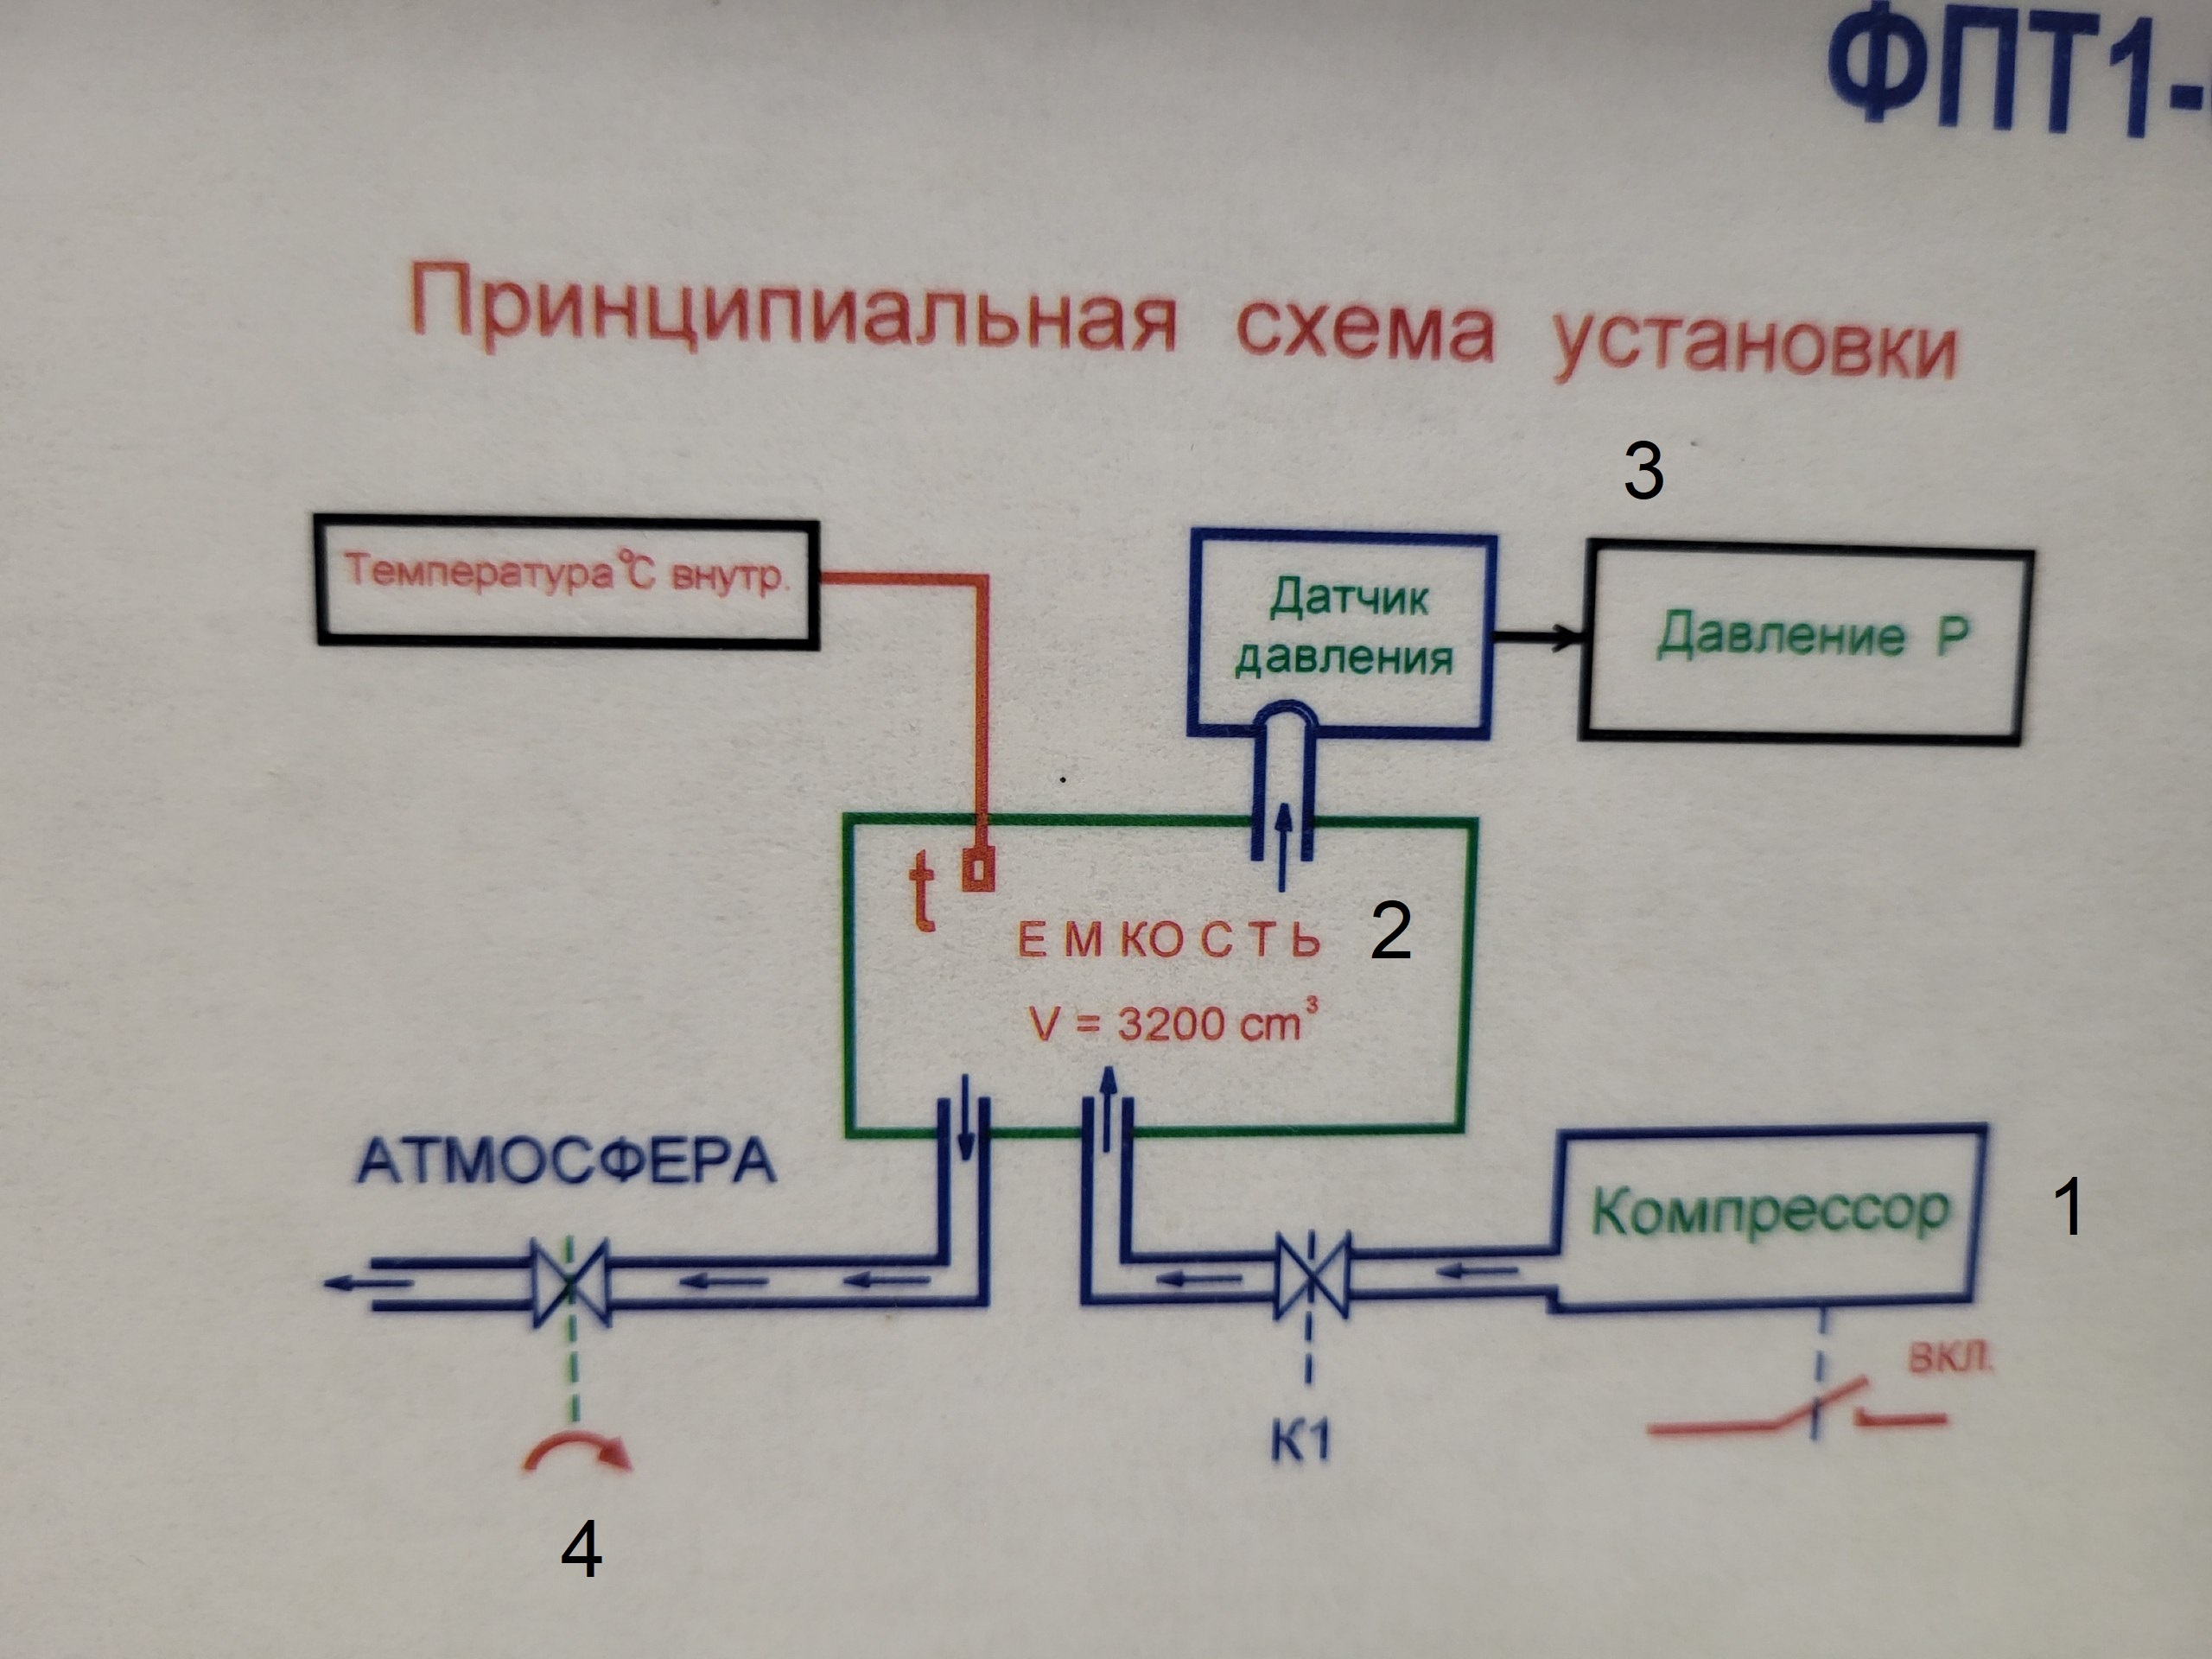
\includegraphics[width=0.8\linewidth]{scheme.jpg}
   \caption{Схема установки}
\end{figure}

\section{Данные прямых измерений, табличные значения}
\begin{table}[H]
   \centering
   \begin{tabular}{|c|c|} \hline
       $P_2$, кПа & $P_1$, кПа\\\hline
$9.4$ & $2.1$\\\hline
$9.4$ & $2.1$\\\hline
$8.0$ & $1.8$\\\hline
$8.0$ & $1.9$\\\hline
$5.9$ & $1.3$\\\hline
$5.9$ & $1.3$\\\hline
$4.1$ & $0.8$\\\hline
$4.1$ & $0.9$\\\hline
   \end{tabular}
   \caption{Данные прямых измерений разности давлений}
\end{table}

Погрешности прямых измерений давления:
\begin{gather*}
    \Delta P = 0.1 \text{ кПа}
\end{gather*}

Количество измерений и коэффициент Стьюдента:
\begin{gather*}
    N = 8\\
    t_{ 0.95 , 8} = 2.365
\end{gather*}

\section{Расчёты и графики}
\begin{table}[H]
   \centering
   \begin{tabular}{|c|c|} \hline
       $\gamma_i$ & $\gamma$\\\hline
$1.29$ & \multirow{8}{*}{1.28}\\\cline{1-1}
$1.29$ & \\\cline{1-1}
$1.29$ & \\\cline{1-1}
$1.31$ & \\\cline{1-1}
$1.28$ & \\\cline{1-1}
$1.28$ & \\\cline{1-1}
$1.24$ & \\\cline{1-1}
$1.28$ & \\\hline
   \end{tabular}
   \caption{Вычисленные значения показателей адиабаты}
\end{table}

Пример вычисления:
\begin{gather*}
    \gamma_1 = \frac{ 9.4}{ 9.4 - 2.1} \approx 1.29
\end{gather*}

Погрешность $\gamma$
\begin{gather*}
    \Delta \gamma_\text{сл} = 2.365 \cdot \sqrt{\frac{ 0.00256}{ 8\cdot7}}\approx0.016\\
    \Delta \gamma_\text{сист} = 1.28\cdot\sqrt{\bigg(0.1 \cdot \bigg(
        \frac{ 1}{ 6.85} + \frac{ 1}{ 6.85 - 1.53}
        \bigg)\bigg)^2 + \bigg(0.1 \cdot \bigg(
        \frac{ 1}{ 6.85 - 1.53}
        \bigg)\bigg)^2}\approx 0.05\\
    \Delta \gamma = \sqrt{(0.016)^2 + ( \frac{ 2}{ 3}\cdot0.05)^2}\approx 0.04
\end{gather*}

\section{Результаты и выводы}
Полученное значение $\gamma = 1.28 \pm 0.04$ близко к табличному ($\gamma_\text{табл}\approx1.40$) но не совпадает с ним.
Это могло получиться из-за того, что соединение баллона с атмосферой не было адиабатным и мог произойти теплообмен, и давление $P_1$ ниже чем предполагаемое в теоретической модели.
Так же это могло получиться из-за того, что после выключения компрессора было выждано недостаточно времени и газ ещё не успел остыть давление $P_2$ снято слишком рано и тоже меньше, чем в теоретической модели.
Оба этих фактора занижают полученное значение $\gamma$.  

\clearpage
\begin{figure}[H]
   \centering
    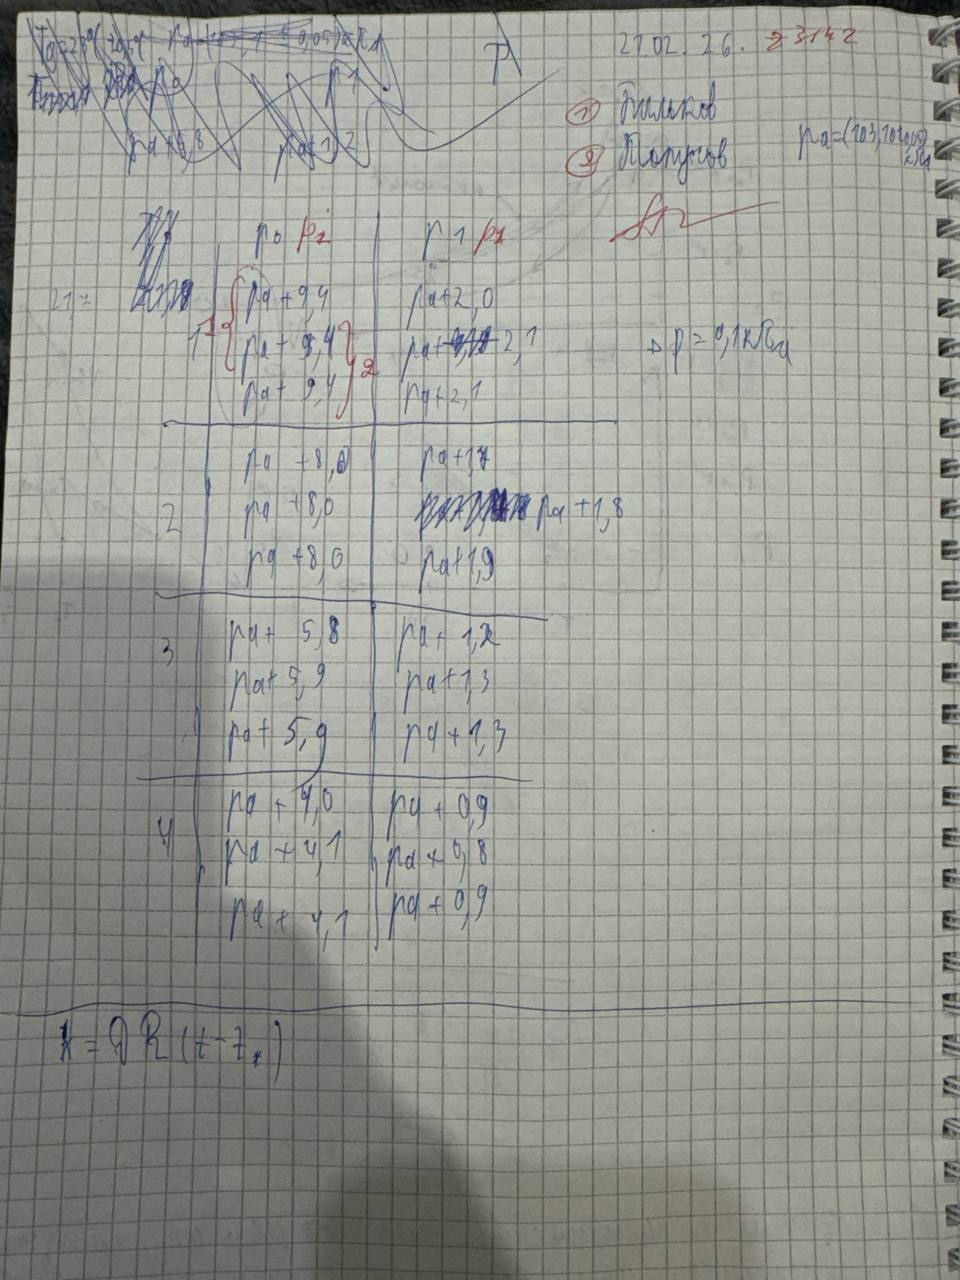
\includegraphics[width=0.8\linewidth]{res.jpg}
   \caption{Подписанне пряме измерения}
\end{figure}
\end{document}